\chapter{Robotik}
\section{Die Welt der Roboter}\label{ch:K09_Robotik}

Roboter sind computergesteuerte Maschinen, die Aufgaben selbstständig
oder teilweise autonom ausführen können. Sie werden unter anderem in
der Industrie, Medizin, Forschung und im Alltag eingesetzt.
Mithilfe von Sensoren erfassen Roboter Informationen über ihre
Umgebung und können darauf reagieren. Ihre Aktionen werden durch
Computerprogramme gesteuert, die auf einem eingebauten Computer,
dem sogenannten Mikrocontroller, ausgeführt werden.
Moderne Roboter können zudem Daten austauschen und ihr Verhalten
mithilfe von Lernverfahren anpassen. Die Vernetzung solcher Geräte
ist ein wichtiger Bestandteil des \emph{Internet of Things} (IoT).

In diesem Kapitel lernen Sie die Grundlagen der Roboterprogrammierung
kennen. Dazu verwenden wir einen Roboter mit einem \emph{micro:bit}
als Mikrocontroller und programmieren ihn mit Python.


\subsection*{Welche Technik steckt hinter einem Roboter?}

Das Herzstück eines Roboters ist ein \emph{Mikrocontroller},
der einen Mikroprozessor enthält und die Steuerung übernimmt.
Er führt Programme aus, verarbeitet Sensordaten und steuert
die aktiven Komponenten des Roboters.

\begin{mydefinition}
    \textbf{Sensoren} erfassen physikalische Grössen wie
    Helligkeit, Abstand oder Temperatur und wandeln diese
    in elektrische Signale um.

    \textbf{Aktoren} setzen elektrische Steuersignale in
    physikalische Wirkungen um, beispielsweise Bewegungen
    durch Motoren, Licht durch LEDs oder Töne durch Lautsprecher.
\end{mydefinition}

Das Zusammenspiel dieser Komponenten bildet die Grundlage
der Robotersteuerung: Sensoren liefern Informationen über
die Umgebung, der Mikrocontroller verarbeitet diese anhand
eines Programms und steuert die Aktoren entsprechend.
Bei unseren Robotern übernimmt der \emph{micro:bit}
die Aufgabe des Mikrocontrollers.

\begin{center}
    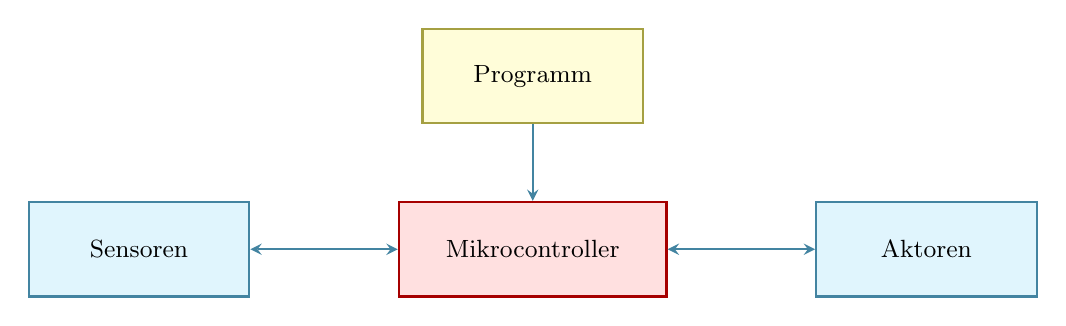
\begin{tikzpicture}[
            >=stealth,
            block/.style={
                    draw,
                    thick,
                    minimum height=1.2cm,
                    align=center,
                    font=\small
                },
            sensor/.style={block, fill=cyan!12, draw=cyan!60!black,
                    minimum width=2.8cm},
            controller/.style={block, fill=red!12, draw=red!65!black,
                    minimum width=3.4cm},
            programm/.style={block, fill=yellow!15, draw=yellow!60!black,
                    minimum width=2.8cm},
            pfeil/.style={->, thick, draw=cyan!60!black}
        ]

        \node[controller] (cpu) at (0,0) {Mikrocontroller};
        \node[sensor] (sens) at (-5,0) {Sensoren};
        \node[sensor] (akt) at (5,0) {Aktoren};
        \node[programm] (prog) at (0,2.2) {Programm};

        \draw[<->, thick, cyan!60!black]
        (sens.east) -- (cpu.west);

        \draw[<->, thick, cyan!60!black]
        (cpu.east) -- (akt.west);

        \draw[pfeil] (prog.south) -- (cpu.north);

    \end{tikzpicture}
\end{center}

Die Programme werden in der Regel auf einem Computer geschrieben und anschliessend auf den Microcontroller geladen. Dieser agiert danach autonom als intelligentess System,
weil er abhängig von Sensordaten eigene vorprogrammierte Entscheidungen
trifft und entsprechend handelt.


\subsection*{Was ist anders beim Programmieren von Robotern?}

Beim Programmieren von Robotern muss man häufig in
\emph{Zuständen} denken. Ein Roboter kann sich beispielsweise
in den Zuständen \enquote{Vorwärtsfahren}, \enquote{Drehen}
oder \enquote{Stillstand} befinden. Er bleibt in einem Zustand,
bis eine bestimmte Bedingung einen Zustandswechsel auslöst.
Solche Wechsel können durch Sensormessungen gesteuert werden,
sodass der Roboter selbstständig auf seine Umgebung reagiert.

Eine weitere Besonderheit ist die Berücksichtigung der
\emph{physikalischen Realität}. Beispielsweise muss durch
Experimente ermittelt werden, wie lange die Motoren laufen
müssen, damit der Roboter eine bestimmte Strecke zurücklegt.
Auch Sensoren müssen häufig durch Messungen \emph{kalibriert}
werden, um ihre Werte richtig interpretieren zu können.
Das wiederholte Testen und Anpassen von Programmen ist
deshalb ein wesentlicher Bestandteil der Robotik.


\subsection*{Inbetriebnahme des Roboters}

Unser Roboter besteht aus einem \emph{micro:bit}, der auf
einem \emph{Maqueen}-Fahrwerk montiert ist. Die Programme
schreiben wir in Python und übertragen sie über ein
USB-Kabel auf den micro:bit.


\begin{myremark}
    Für die Programmierung verwenden wir in diesem Kapitel
    die Webseite \url{https://webtigerpython.ethz.ch}
    anstelle von VS Code. Diese stellt die benötigten
    Robotik-Bibliotheken bereits zur Verfügung und bietet
    einen nützlichen Simulator, mit dem viele Programme
    getestet werden können, bevor man sie auf den
    Roboter überträgt.

    Damit Programme direkt aus dem Browser auf den Roboter
    übertragen werden können, muss der Browser die
    Schnittstelle \emph{WebUSB} unterstützen. Dies ist
    beispielsweise bei Chrome, Edge und Opera der Fall,
    nicht jedoch bei Safari oder Firefox.
\end{myremark}





\begin{enumerate}
    \item Stecken Sie den micro:bit in die dafür vorgesehene
          Steckleiste des Maqueen-Fahrwerks. Achten Sie
          auf die korrekte Ausrichtung.

    \item Verbinden Sie den micro:bit über ein USB-Datenkabel
          mit Ihrem Computer. Achtung: Sobald der micro:bit mit Strom versogt wird, startet, das zuletzt geladen Programm. Halten Sie den Roboter fest, damit er nicht versehentlich vom Tisch fährt!

    \item Öffnen Sie im Browser Google Chrome die Webseite
          \url{https://webtigerpython.ethz.ch}.

    \item Wählen Sie in den Einstellungen als Gerät
          \emph{micro:bit} aus.

    \item Verbinden Sie den micro:bit über die
          Verbindungsfunktion der Entwicklungsumgebung
          mit dem Browser. Wählen Sie das angeschlossene
          Gerät aus und bestätigen Sie die Verbindung.

    \item Geben Sie das folgende Programm im Editor ein:

          \begin{lstlisting}[language=Python]
from mbrobot import *

setLED(1)
delay(2000)
setLED(0)
\end{lstlisting}

    \item Übertragen Sie das Programm mit der entsprechenden
          Schaltfläche auf den micro:bit (Flash).
          Warten Sie, bis die Übertragung abgeschlossen ist.

    \item Beobachten Sie die LEDs des Roboters.
          Beide LEDs sollten zwei Sekunden lang leuchten
          und danach wieder erlöschen.
\end{enumerate}

\begin{myremark}
    Mit \texttt{from mbrobot import *} werden sämtliche Befehle aus der Bibliothek für den Micro:bit-Roboter importiert.

    Der Befehl \texttt{setLED(1)} schaltet die beiden
    LEDs des Maqueen ein, während \texttt{setLED(0)}
    sie wieder ausschaltet.

    Mit \texttt{delay(2000)} wird die Programmausführung
    für 2000 Millisekunden, also zwei Sekunden, unterbrochen.

    Der Micro:bit verfügt neben der USB-Büchse einen reset-Knopf, mit dem man das Programm neu starten kann. Probieren Sie es!
\end{myremark}


\section{Der fahrende Roboter}

Die Bibliothek \texttt{mbrobot} stellt verschiedene Befehle
zur Steuerung des Roboters zur Verfügung. Mit
\texttt{forward()} und \texttt{backward()} fährt der Roboter
vorwärts bzw. rückwärts. Die Befehle \texttt{left()} und
\texttt{right()} lassen ihn auf der Stelle drehen, während
\texttt{leftArc(radius)} und \texttt{rightArc(radius)}
eine Kurvenfahrt mit dem angegebenen Radius ermöglichen.
Mit \texttt{stop()} werden die Motoren angehalten.



\begin{myexercise}

    Der Roboter soll während zwei Sekunden vorwärtsfahren,
    sich anschliessend um \(90^\circ\) nach links drehen,
    erneut zwei Sekunden vorwärtsfahren und schliesslich
    anhalten.

    Das folgende Programm soll diese Bewegung ausführen:

    \begin{lstlisting}[language=Python]
from mbrobot import *

forward()
delay(2000)
left()
delay(550)
forward()
delay(2000)
stop()
    \end{lstlisting}

    Die Dauer der Drehung wurde zunächst auf
    \(\SI{550}{\milli\second}\) festgelegt. Ob sich der
    Roboter in dieser Zeit tatsächlich um \(90^\circ\)
    dreht, hängt unter anderem von der Geschwindigkeit
    der Motoren und der Beschaffenheit des Untergrunds ab.

    \begin{enumerate}
        \item Übertragen Sie das Programm auf den Roboter
              und beobachten Sie seine Bewegung.

        \item Verändern Sie die Dauer der Drehung so lange,
              bis sich der Roboter möglichst genau um
              \(90^\circ\) dreht.

        \item Wie lange muss sich der Roboter ungefähr
              drehen, damit er eine vollständige
              Drehung um \(360^\circ\) ausführt?
              Überprüfen Sie Ihre Vermutung experimentell.
    \end{enumerate}

    \begin{myanswer}
        Die benötigte Zeit für eine Drehung um \(90^\circ\)
        muss experimentell bestimmt werden und hängt
        vom verwendeten Roboter ab.

        Für eine Drehung um \(360^\circ\) benötigt der
        Roboter bei konstanter Drehgeschwindigkeit
        ungefähr die vierfache Zeit.
    \end{myanswer}
\end{myexercise}


\begin{myremark}

    Beim \emph{Kalibrieren} werden die Einstellungen eines
    Geräts mithilfe von Messungen überprüft und gegebenenfalls
    angepasst, damit es möglichst genau wie gewünscht
    funktioniert.

    Bei unserem Roboter muss beispielsweise experimentell
    bestimmt werden, wie lange die Motoren laufen müssen,
    damit er sich um einen bestimmten Winkel dreht oder
    eine bestimmte Strecke zurücklegt. Auch Sensoren müssen
    häufig kalibriert werden, damit ihre Messwerte korrekt
    interpretiert werden können.

    Da das Verhalten eines Roboters von äusseren Einflüssen
    wie der Beschaffenheit des Untergrunds oder dem
    Ladezustand der Batterie abhängt, kann eine erneute
    Kalibrierung notwendig sein.
\end{myremark}


\begin{myexercise}

    Erstellen Sie mithilfe von Gegenständen auf dem Boden
    einen Parcours wie in der folgenden Abbildung.

    \begin{center}
        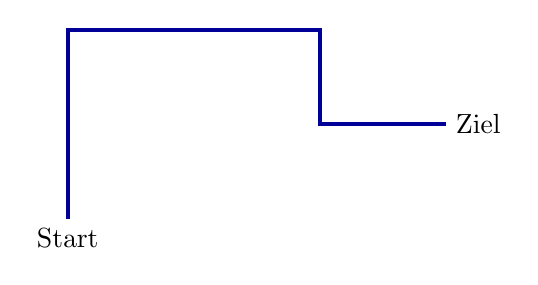
\begin{tikzpicture}[scale=0.8, thick]
            \draw[blue!60!black, line width=1.5pt]
            (0,0) -- (0,3) -- (4,3) -- (4,1.5) -- (6,1.5);

            \node[below] at (0,0) {Start};
            \node[right] at (6,1.5) {Ziel};
        \end{tikzpicture}
    \end{center}

    Schreiben Sie ein Programm, das den Roboter möglichst
    genau vom Start bis zum Ziel fahren lässt.
    Verwenden Sie dazu die bekannten Bewegungsbefehle
    und geeignete Wartezeiten.

    Testen Sie Ihr Programm mehrfach und passen Sie
    die Fahr- und Drehzeiten so lange an, bis der
    Roboter den Parcours möglichst genau abfährt.

    \begin{myanswer}
        Individuelle Lösung. Der Roboter muss zunächst
        geradeaus fahren, sich um \(90^\circ\) nach rechts
        drehen, erneut geradeaus fahren, sich nochmals
        um \(90^\circ\) nach rechts drehen und schliesslich
        nach einer weiteren Geradeausfahrt anhalten.
        Die Fahr- und Drehzeiten müssen experimentell
        bestimmt werden.
    \end{myanswer}
\end{myexercise}


\begin{myexercise}

    Mit dem Befehl \texttt{setAlarm(1)} kann der Roboter
    einen Signalton einschalten, mit \texttt{setAlarm(0)}
    wird dieser wieder ausgeschaltet. Dazu muss die
    Bibliothek \texttt{mbalarm} importiert werden.

    Schreiben Sie ein Programm, das die folgenden
    Aktionen ausführt:

    \begin{enumerate}
        \item Der Roboter fährt während drei Sekunden
              vorwärts. Gleichzeitig sollen die beiden
              LEDs zweimal ein- und ausgeschaltet werden.

        \item Anschliessend fährt der Roboter während
              drei Sekunden rückwärts. Während dieser
              Zeit soll der Signalton eingeschaltet sein.

        \item Zum Schluss hält der Roboter an und
              schaltet den Signalton aus.
    \end{enumerate}

    \begin{myanswer}
        \begin{lstlisting}[language=Python]
from mbrobot import *
from mbalarm import *

# Vorwaertsfahren und zweimal blinken
forward()
for _ in range(2):
    setLED(1)
    delay(750)
    setLED(0)
    delay(750)

# Rueckwaertsfahren mit Signalton
backward()
setAlarm(1)
delay(3000)

# Anhalten und Alarm ausschalten
stop()
setAlarm(0)
        \end{lstlisting}
    \end{myanswer}
\end{myexercise}



\begin{myexercise}

    Stellen Sie drei Gegenstände (z.\,B. Flaschen)
    gemäss der folgenden Abbildung auf dem Boden auf.

    \begin{center}
        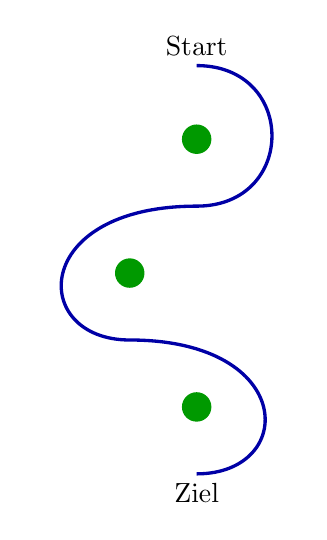
\begin{tikzpicture}[scale=0.85]
            % Hindernisse
            \fill[green!60!black] (0.5,4) circle (0.22);
            \fill[green!60!black] (-0.5,2) circle (0.22);
            \fill[green!60!black] (0.5,0) circle (0.22);

            % Slalomstrecke
            \draw[blue!65!black, very thick]
            (0.5,5.1)
            .. controls (2.0,5.1) and (2.0,3.0) ..
            (0.5,3.0)
            .. controls (-2.0,3.0) and (-2.0,1.0) ..
            (-0.5,1.0)
            .. controls (2.0,1.0) and (2.0,-1.0) ..
            (0.5,-1.0);

            \node[above] at (0.5,5.1) {Start};
            \node[below] at (0.5,-1.0) {Ziel};
        \end{tikzpicture}
    \end{center}

    Schreiben Sie ein Programm, mit dem der Roboter
    die Slalomstrecke möglichst schnell abfährt,
    ohne die Hindernisse zu berühren.

    Experimentieren Sie mit den Fahrzeiten,
    Drehwinkeln und Geschwindigkeiten, um
    eine möglichst schnelle und präzise
    Fahrt zu erreichen.

    \textbf{Hinweis:}
    Mit dem Befehl \texttt{setSpeed(n)} können Sie
    die Geschwindigkeit des Roboters einstellen.
    Dabei ist \texttt{n} eine Zahl zwischen
    \(0\) und \(100\), wobei \(100\) der maximalen
    Geschwindigkeit entspricht.

    \begin{myanswer}
        Individuelle Lösung. Die Fahrzeiten und
        Geschwindigkeiten müssen experimentell
        bestimmt und an den Parcours angepasst werden.
    \end{myanswer}
\end{myexercise}


\subsection*{Schleifen}
Roboter sind besonders dann sinnvoll einsetzbar, wenn mehrere Tätigkeiten
mit identischen Abläufen ausgeführt werden müssen. Für Menschen sind solche
Tätigkeiten sehr monoton und der Roboter kann sie in der Regel effizienter
erledigen.


\begin{myexercise}

    \begin{center}
        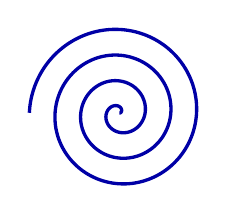
\begin{tikzpicture}[scale=0.65]
            \draw[blue!65!black, very thick,
                domain=0:7*pi, samples=350,
                smooth, variable=\t]
            plot ({0.08*\t*cos(\t r)},
                {0.08*\t*sin(\t r)});
        \end{tikzpicture}
    \end{center}

    \begin{enumerate}
        \item Schreiben Sie ein Programm, mit dem der Roboter
              eine Spirale von innen nach aussen abfährt.
              Verwenden Sie dazu eine \texttt{while} oder \texttt{for}-Schleife
              und vergrössern Sie nach jedem Schleifendurchlauf
              den Radius im Befehl \texttt{leftArc(radius)}.

        \item Der Roboter soll nun eine Spirale von aussen
              nach innen abfahren. Beginnen Sie mit einem
              Radius von \(\SI{30}{\centi\meter}\) und
              verkleinern Sie diesen nach jeder Runde.
              Nach neun Runden soll sich der Roboter
              auf der Stelle drehen.
    \end{enumerate}


    \begin{myanswer}
        Die Fahrzeiten müssen experimentell angepasst werden.

        \textbf{a) Von innen nach aussen}

        \begin{lstlisting}[language=Python]
from mbrobot import *

for i in range(10):
    radius = 5 + 3 * i
    leftArc(radius)
    delay(2000)

stop()
    \end{lstlisting}

        \textbf{b) Von aussen nach innen}

        \begin{lstlisting}[language=Python]
from mbrobot import *

for i in range(9):
    radius = 30 - 3 * i
    leftArc(radius)
    delay(2000)

left()
    \end{lstlisting}
    \end{myanswer}

\end{myexercise}


\begin{myexercise}
    Ein Roboter soll Material aus einem Lager L zu den
    drei Standorten A, B und C transportieren. Dabei
    fährt er zunächst vom Lager zum Standort A und
    anschliessend wieder zurück zum Lager. Danach
    beliefert er auf die gleiche Weise die Standorte
    B und C. Diesen Ablauf wiederholt er unendlich oft.

    \begin{center}
        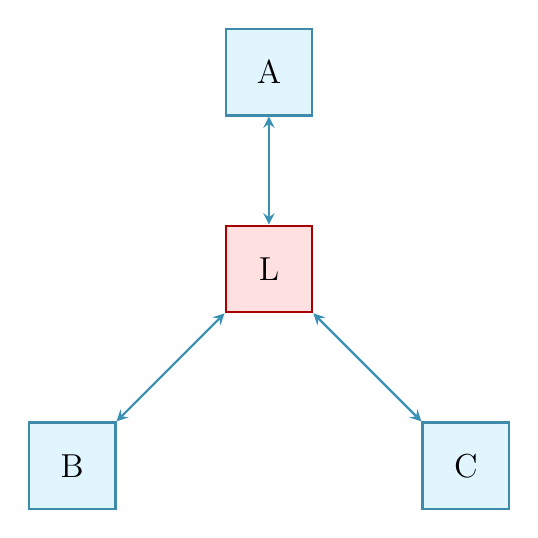
\begin{tikzpicture}[
                >=stealth,
                standort/.style={
                        draw=cyan!65!black,
                        fill=cyan!12,
                        thick,
                        minimum width=1.1cm,
                        minimum height=1.1cm,
                        font=\large
                    },
                lager/.style={
                        standort,
                        draw=red!65!black,
                        fill=red!12
                    }
            ]
            \node[lager] (L) at (0,0) {L};
            \node[standort] (A) at (0,2.5) {A};
            \node[standort] (B) at (-2.5,-2.5) {B};
            \node[standort] (C) at (2.5,-2.5) {C};

            \draw[<->, thick, cyan!70!black]
            (L.north) -- (A.south);
            \draw[<->, thick, cyan!70!black]
            (L.south west) -- (B.north east);
            \draw[<->, thick, cyan!70!black]
            (L.south east) -- (C.north west);
        \end{tikzpicture}
    \end{center}

    Schreiben Sie ein Programm, das diese Transportfahrten
    automatisch ausführt. Verwenden Sie dazu eine
    \texttt{while True}-Schleife.

    Kalibrieren Sie die benötigten Fahr- und Drehzeiten
    so, dass der Roboter die Standorte möglichst genau
    erreicht. Nehmen Sie an, dass das Be- und Entladen
    jeweils zwei Sekunden dauert.

    \begin{myanswer}
        Eine mögliche Lösung besteht darin, für die
        Transportfahrten eine eigene Funktion zu definieren.
        Der Roboter startet im Lager und ist zunächst
        in Richtung A ausgerichtet.

        \begin{lstlisting}[language=Python]
from mbrobot import *

# Zeiten muessen kalibriert werden!
FAHRZEIT = 2000
DREHZEIT_120 = 730

while True:
    ### Transport
    delay(2000)       # Beladen
    forward()
    delay(FAHRZEIT)
    stop()
    delay(2000)       # Entladen
    backward()
    delay(FAHRZEIT)
    stop()
    
    ### Auf das naechste Ziel ausrichten            
    left()
    delay(DREHZEIT_120)
    stop()
        \end{lstlisting}

        Die Lösung setzt voraus, dass die drei Standorte
        im Winkelabstand von jeweils \(120^\circ\) um
        das Lager angeordnet sind und alle denselben
        Abstand zum Lager haben. Die angegebenen Zeiten
        sind lediglich Beispielwerte und müssen
        experimentell bestimmt werden.
    \end{myanswer}
\end{myexercise}



\subsection*{Eigene Befehle definieren}




Wie bei gewöhnlichen Python-Programmen können auch für
den Roboter eigene Funktionen definiert und Schleifen
verwendet werden. Das folgende Programm definiert eine
Funktion \texttt{blink()}, die die LEDs kurz aufleuchten
lässt. Anschliessend werden verschiedene Bewegungsbefehle
in einer Schleife viermal wiederholt.

\begin{lstlisting}[language=Python]
from mbrobot import *

def blink():
    setLED(1)
    delay(500)
    setLED(0)
    delay(500)

for _ in range(4):
    forward()
    delay(2000)
    stop()
    blink()
    blink()
    backward()
    delay(2000)
    left()
    delay(550)
    stop()
\end{lstlisting}

\begin{myexercise}
    Beschreiben Sie möglichst genau, welche Bewegungen
    der Roboter beim Ausführen des obigen Programms macht
    und wann seine LEDs aufleuchten.

    \begin{myanswer}
        Der Roboter wiederholt viermal die folgende
        Befehlsfolge:
        \begin{enumerate}
            \item Er fährt zwei Sekunden vorwärts und hält an.
            \item Die LEDs blinken zweimal.
            \item Er fährt zwei Sekunden rückwärts.
            \item Er dreht sich während 550 Millisekunden
                  nach links und hält an.
        \end{enumerate}
        Die tatsächlichen Strecken und Drehwinkel hängen
        unter anderem von der Geschwindigkeit der Motoren
        und der Beschaffenheit des Untergrunds ab.
    \end{myanswer}
\end{myexercise}


\begin{myexercise}


    Der Roboter soll die folgende treppenähnliche Strecke
    abfahren. Jede Stufe besteht aus zwei gleich langen
    geraden Strecken.

    \begin{center}
        \begin{tikzpicture}[scale=0.8]
            \draw[blue!65!black, very thick]
            (0,0) -- (0,1.5) -- (1.5,1.5)
            -- (1.5,3) -- (3,3)
            -- (3,4.5) -- (4.5,4.5);
            \node[below] at (0,0) {Start};
            \node[right] at (4.5,4.5) {Ziel};
        \end{tikzpicture}
    \end{center}

    Schreiben Sie ein Programm, das den Roboter
    vom Start zum Ziel fahren lässt.
    Definieren Sie dazu eine Funktion
    \texttt{step()}, die den Roboter eine
    vollständige Stufe fahren lässt.
    Rufen Sie diese Funktion dreimal auf.
    Nach jeder Stufe soll der Roboter einmal
    mit seinen LEDs blinken.


    \begin{myanswer}
        Die folgenden Programme zeigen mögliche Lösungen.
        Die Fahr- und Drehzeiten müssen experimentell
        kalibriert werden. Wir nehmen an, dass eine
        Drehung um \(90^\circ\) etwa 550 ms dauert.


        \begin{lstlisting}[language=Python]
from mbrobot import *

def step():
    forward()
    delay(1000)
    right()
    delay(550)
    forward()
    delay(1000)
    left()
    delay(550)
    stop()

def blink():
    setLED(1)
    delay(500)
    setLED(0)

# Roboter startet in Richtung oben
for _ in range(3):
    step()
    blink()
        \end{lstlisting}
    \end{myanswer}
\end{myexercise}
















\section{Sensoren}

Sensoren sind aus unserem Alltag nicht mehr wegzudenken und kommen
beispielsweise in Smartphones, Autos und Haushaltsgeräten zum Einsatz.
Sie messen physikalische oder chemische Grössen wie Temperatur,
Abstand oder Helligkeit und wandeln diese in elektrische Signale um.
In einem \emph{Regelkreis} werden die gemessenen Sensorwerte mit
vorgegebenen Sollwerten verglichen, um entsprechende Aktionen auszulösen.
Da Sensorwerte häufig ungenau sind und von den Umgebungsbedingungen
beeinflusst werden, müssen diese Unsicherheiten bei der Programmierung
berücksichtigt werden.
Mithilfe von Variablen und bedingten Anweisungen können Roboter
Sensorwerte auswerten und selbstständig auf ihre Umgebung reagieren.


\subsection*{Distanzen messen mit Ultraschall}

Mit einem \emph{Ultraschallsensor} lässt sich die Distanz zu einem
Objekt messen. Der Sensor besitzt einen Sender (S) und einen
Empfänger (E) für Schallwellen. Der Sender erzeugt einen kurzen
Ultraschallimpuls, der von einem Objekt reflektiert und anschliessend
vom Empfänger registriert wird.

Dabei wird die Zeit gemessen, die der Schallimpuls für den Weg
vom Sender zum Objekt und wieder zurück zum Empfänger benötigt.
Dieses Verfahren nennt man \emph{Puls-Laufzeit-Messung}.

\begin{center}
    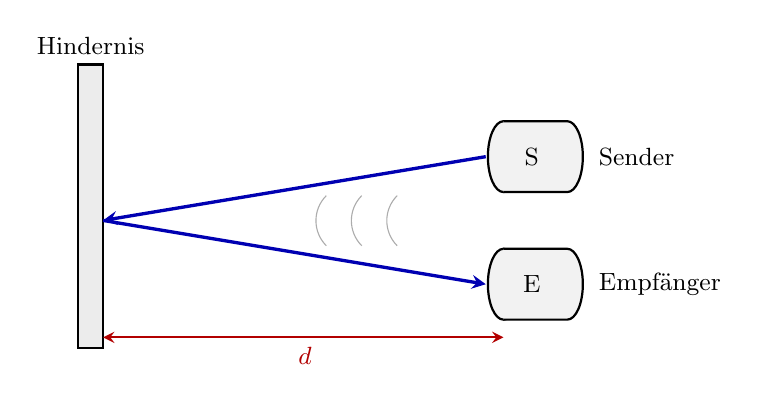
\begin{tikzpicture}[
            >=stealth,
            thick,
            scale=0.9,
            every node/.style={font=\small}
        ]
        % Hindernis
        \draw[fill=gray!15] (0,-1.8) rectangle (0.35,2.2);
        \node[above] at (0.175,2.2) {Hindernis};

        % Sender
        \draw[fill=gray!10]
        (6,0.9) ellipse (0.22 and 0.5);
        \draw[fill=gray!10]
        (6,0.4) -- (6.9,0.4)
        arc[start angle=-90,end angle=90,
                x radius=0.22,y radius=0.5]
        -- (6,1.4);
        \node at (6.4,0.9) {S};

        % Empfaenger
        \draw[fill=gray!10]
        (6,-0.9) ellipse (0.22 and 0.5);
        \draw[fill=gray!10]
        (6,-1.4) -- (6.9,-1.4)
        arc[start angle=-90,end angle=90,
                x radius=0.22,y radius=0.5]
        -- (6,-0.4);
        \node at (6.4,-0.9) {E};

        % Schallwege
        \draw[->, blue!70!black, very thick]
        (5.75,0.9) -- (0.35,0);
        \draw[->, blue!70!black, very thick]
        (0.35,0) -- (5.75,-0.9);

        % Schallwellen
        \foreach \x in {3.5,4,4.5} {
                \draw[gray!65, thin]
                (\x,0.35) arc[start angle=135,
                        end angle=225,radius=0.5];
            }

        % Distanz
        \draw[<->, red!70!black, thick]
        (0.35,-1.65) -- (6,-1.65);
        \node[below, red!70!black] at (3.2,-1.65) {\(d\)};

        \node[right] at (7.2,0.9) {Sender};
        \node[right] at (7.2,-0.9) {Empfänger};
    \end{tikzpicture}

    \smallskip
    \small Puls-Laufzeit-Messung mit einem Ultraschallsensor
\end{center}

Da der Schall die Strecke zum Hindernis und wieder zurück
zurücklegt, ergibt sich für die Distanz \(d\):

\[
    d = \frac{v \cdot t}{2}
\]

Dabei bezeichnet \(v\) die Schallgeschwindigkeit
(etwa \(\SI{343}{\meter\per\second}\) bei Raumtemperatur)
und \(t\) die gemessene Laufzeit des Ultraschallimpulses.

Unser Maqueen-Roboter verfügt über einen Ultraschallsensor,
mit dem sich Distanzen zu Hindernissen messen lassen.
Mit der Funktion \texttt{getDistance()} kann die aktuelle
Distanz abgefragt werden:

\begin{lstlisting}[language=Python]
from mbrobot import *
while True:
    distanz = getDistance()
    print(distanz)
    delay(100)
\end{lstlisting}

Probieren Sie das Programm oben aus.
Die Funktion \texttt{getDistance()} gibt die gemessene
Distanz in Zentimetern zurück. Der nutzbare Messbereich
liegt ungefähr zwischen \(\SI{3}{\centi\meter}\) und
\(\SI{250}{\centi\meter}\). Wenn der Sensor kein Hindernis erkennt, wird der Wert 255 zurückgegeben. Der \texttt{delay}-Befehl ist nötig, damit die einzelnen Messungen sich nicht überschneiden, schliesslich benötigt die Messung und deren Verarbeitung etwas Zeit.

% \begin{myremark}
%     Ultraschallsensoren liefern nicht immer zuverlässige
%     Messwerte. Insbesondere bei schrägen, sehr kleinen
%     oder schallabsorbierenden Oberflächen kann die Messung
%     ungenau sein oder ganz fehlschlagen.
% \end{myremark}


\begin{myexample}


    In einem \emph{Regelungssystem} wird ein Roboter so gesteuert,
    dass er einen vorgegebenen \emph{Sollwert} möglichst genau
    einhält. Dazu misst er mithilfe seiner Sensoren regelmässig
    den aktuellen \emph{Istwert} und passt sein Verhalten
    entsprechend der Abweichung vom Sollwert an.

    Im folgenden Beispiel soll der Roboter den Bewegungen
    einer Hand folgen und dabei stets einen Abstand von
    \(\SI{20}{\centi\meter}\) einhalten. Ist die gemessene
    Distanz kleiner als \(\SI{20}{\centi\meter}\), fährt er
    rückwärts. Ist sie grösser, fährt er vorwärts.
    Die Distanz wird ungefähr alle 100 Millisekunden
    erneut gemessen.

    \begin{lstlisting}[language=Python]
from mbrobot import *

setSpeed(20)

while True:
    d = getDistance()
    if d < 20:
        backward()
    else:
        forward()
    delay(100)
    \end{lstlisting}

    Der Roboter reagiert fortlaufend auf Veränderungen
    des Abstands und versucht so, den Sollwert einzuhalten.
\end{myexample}


\begin{myexercise}
    \textbf{Verbesserung der Abstandsregelung}

    Das Programm aus dem vorherigen Beispiel soll
    schrittweise verbessert werden. Verwenden Sie dazu die \texttt{if-elif-else}-Struktur.

    \begin{enumerate}
        \item Passen Sie das Programm so an, dass der Roboter
              stehen bleibt, wenn der gemessene Abstand
              grösser als \(\SI{50}{\centi\meter}\) ist.
              Damit soll verhindert werden, dass der Roboter
              einer Hand folgt, die sich zu weit entfernt.

              % \item Im bisherigen Programm fährt der Roboter
              %       auch dann weiter, wenn der gewünschte Abstand
              %       von \(\SI{20}{\centi\meter}\) genau erreicht ist.
              %       Ändern Sie das Programm so, dass der Roboter
              %       bei einem Abstand von genau
              %       \(\SI{20}{\centi\meter}\) stehen bleibt.

        \item In der Praxis schwanken die Messwerte des
              Ultraschallsensors leicht. Dadurch kann es
              passieren, dass der Roboter ständig zwischen
              Vorwärts- und Rückwärtsfahren wechselt.

              Bauen Sie deshalb einen \emph{Toleranzbereich}
              ein: Bei einem Abstand zwischen
              \(\SI{18}{\centi\meter}\) und
              \(\SI{22}{\centi\meter}\) soll der Roboter
              stehen bleiben. Ausserhalb dieses Bereichs
              soll er wie bisher reagieren. Die Bedingung
              aus Teilaufgabe 1. soll weiterhin gelten.
    \end{enumerate}

    \begin{myanswer}
        \textbf{a) Maximale Distanz}

        \begin{lstlisting}[language=Python]
from mbrobot import *

setSpeed(20)

while True:
    d = getDistance()
    if d > 50:
        stop()
    elif d < 20:
        backward()
    else:
        forward()
    delay(100)
        \end{lstlisting}

        %         \textbf{b) Anhalten beim Sollwert}

        %         \begin{lstlisting}[language=Python]
        % from mbrobot import *

        % setSpeed(20)

        % while True:
        %     d = getDistance()
        %     if d > 50:
        %         stop()
        %     elif d < 20:
        %         backward()
        %     elif d > 20:
        %         forward()
        %     else:
        %         stop()
        %     delay(100)
        %         \end{lstlisting}

        \textbf{c) Toleranzbereich}

        \begin{lstlisting}[language=Python]
from mbrobot import *

setSpeed(20)

while True:
    d = getDistance()
    if d > 50:
        stop()
    elif d < 18:
        backward()
    elif d > 22:
        forward()
    else:
        stop()
    delay(100)
        \end{lstlisting}

        Der Roboter bleibt nun stehen, wenn der Abstand
        zwischen 18 und 22 cm liegt oder grösser als
        50 cm ist. Dadurch werden unnötige
        Richtungswechsel in der Nähe des Sollwerts
        reduziert.
    \end{myanswer}
\end{myexercise}



\begin{myexercise}
    \textbf{Annäherung an ein Hindernis}

    Stellen Sie ein Hindernis in einem Abstand von ungefähr
    \(\SI{50}{\centi\meter}\) vor den Roboter.

    Schreiben Sie ein Programm, das den Roboter mit einer
    Geschwindigkeit von 15 vorwärtsfahren lässt und dabei
    alle \(\SI{100}{\milli\second}\) die Distanz zum Hindernis misst.

    Sobald die gemessene Distanz kleiner als
    \(\SI{20}{\centi\meter}\) ist, soll der Roboter einen
    Signalton einschalten. Unterschreitet die Distanz
    \(\SI{10}{\centi\meter}\), soll der Roboter anhalten
    und den Signalton ausschalten.

    \begin{myanswer}
        \begin{lstlisting}[language=Python]
from mbrobot import *
from mbalarm import *

setSpeed(15)
forward()

while True:
    d = getDistance()

    if d < 10:
        stop()
        setAlarm(0)
        break
    elif d < 20:
        setAlarm(1)

    delay(100)
        \end{lstlisting}

        Die Bedingung \texttt{d < 10} muss zuerst geprüft
        werden, da bei einer Distanz unter 10 cm auch
        die Bedingung \texttt{d < 20} erfüllt ist.
        Mit \texttt{break} wird die Schleife beendet,
        sobald der Roboter angehalten hat.
    \end{myanswer}
\end{myexercise}


\begin{myexercise}
    \textbf{Zwischen zwei Hindernissen pendeln}

    Stellen Sie zwei Hindernisse mit einem Abstand von
    ungefähr einem Meter einander gegenüber auf.
    Platzieren Sie den Roboter dazwischen, sodass
    sein Ultraschallsensor auf eines der Hindernisse zeigt.

    Schreiben Sie ein Programm, das den Roboter
    fortlaufend zwischen den beiden Hindernissen
    hin- und herfahren lässt.

    Sobald die gemessene Distanz zu einem Hindernis
    kleiner als \(\SI{20}{\centi\meter}\) ist,
    soll der Roboter:
    \begin{enumerate}
        \item anhalten,
        \item für eine Sekunde einen Signalton auslösen,
        \item sich um \(180^\circ\) drehen,
        \item und anschliessend in die entgegengesetzte
              Richtung weiterfahren.
    \end{enumerate}

    Verwenden Sie eine \texttt{while True}-Schleife.
    Die benötigte Drehzeit muss experimentell
    kalibriert werden.

    \begin{myanswer}
        \begin{lstlisting}[language=Python]
from mbrobot import *
from mbalarm import *

setSpeed(20)

# Zeit fuer eine Drehung um 180 Grad
DREHZEIT = 1100

forward()

while True:
    d = getDistance()

    if d < 20:
        stop()

        setAlarm(1)
        delay(1000)
        setAlarm(0)

        left()
        delay(DREHZEIT)
        stop()

        forward()

    delay(100)
        \end{lstlisting}

        Der Roboter misst fortlaufend die Distanz zum
        nächsten Hindernis. Sobald diese kleiner als
        20 cm ist, hält er an, gibt einen Signalton
        ab und dreht sich um \(180^\circ\).

        Anschliessend fährt er in die Gegenrichtung.
        Da die gesamte Befehlsfolge in einer
        \texttt{while True}-Schleife steht, wird
        dieser Vorgang unendlich oft wiederholt.

        Die Konstante \texttt{DREHZEIT} muss so
        kalibriert werden, dass sich der Roboter
        möglichst genau um \(180^\circ\) dreht.
    \end{myanswer}
\end{myexercise}


\begin{myexercise}
    \textbf{Der Roboter sucht den Ausgang}

    Ein Roboter mit einem Ultraschallsensor befindet sich
    in einem Raum mit einem Ausgang. Seine Aufgabe besteht
    darin, den Ausgang selbstständig zu finden und den
    Raum zu verlassen.

    \begin{center}
        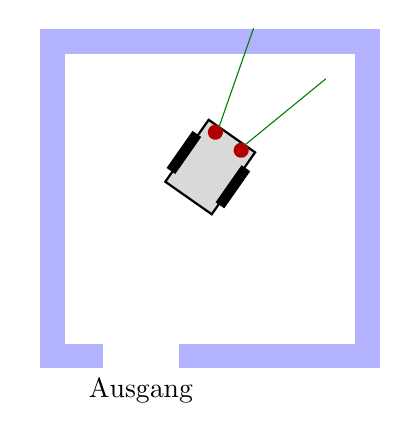
\begin{tikzpicture}[scale=0.8]
            % Raum mit Ausgang
            \draw[blue!30, line width=9pt]
            (0,0) -- (0,5) -- (5,5) -- (5,0) -- (2,0);
            \draw[blue!30, line width=9pt]
            (-0.2,0) -- (0.8,0);

            % Roboter
            \begin{scope}[shift={(2.5,3)}, rotate=-35]
                \draw[fill=gray!30, thick]
                (-0.45,-0.6) rectangle (0.45,0.6);
                \draw[fill=black]
                (-0.55,-0.4) rectangle (-0.4,0.3);
                \draw[fill=black]
                (0.4,-0.4) rectangle (0.55,0.3);
                \fill[red!70!black] (-0.25,0.5) circle (0.12);
                \fill[red!70!black] (0.25,0.5) circle (0.12);

                % Ultraschall
                \draw[green!50!black, thin]
                (-0.25,0.6) -- (-0.7,2.2);
                \draw[green!50!black, thin]
                (0.25,0.6) -- (0.7,2.2);
            \end{scope}

            \node[below] at (1.4,-0.2) {Ausgang};
        \end{tikzpicture}
    \end{center}

    Bauen Sie mithilfe von Gegenständen einen einfachen
    Raum mit einem Ausgang auf, wie in der Abbildung
    dargestellt.

    Überlegen Sie sich eine Strategie, mit der der Roboter
    den Ausgang mithilfe seines Ultraschallsensors
    selbstständig finden kann. Schreiben Sie ein
    entsprechendes Programm und testen Sie es.

    % \textbf{Hinweis:} Der Roboter könnte sich zunächst
    % auf der Stelle drehen und dabei die Distanzen in
    % verschiedene Richtungen messen. In welcher Richtung
    % könnte sich der Ausgang befinden?

    % \begin{myanswer}
    %         Eine mögliche Strategie besteht darin, die
    %         Umgebung schrittweise abzutasten und anschliessend
    %         in die Richtung mit der grössten gemessenen
    %         Distanz zu fahren.

    %         \begin{lstlisting}[language=Python]
    % from mbrobot import *

    % setSpeed(20)

    % beste_distanz = 0
    % beste_richtung = 0

    % # Umgebung in 36 Richtungen abtasten
    % for i in range(36):
    %     d = getDistance()

    %     if d > beste_distanz:
    %         beste_distanz = d
    %         beste_richtung = i

    %     left()
    %     delay(100)
    %     stop()
    %     delay(100)

    % # In die beste Richtung drehen
    % for _ in range(beste_richtung):
    %     left()
    %     delay(100)
    %     stop()

    % # In Richtung Ausgang fahren
    % forward()
    % delay(3000)
    % stop()
    %         \end{lstlisting}

    %         Die Drehzeiten und die Fahrzeit müssen
    %         experimentell kalibriert werden. Die Lösung
    %         funktioniert nur unter geeigneten Bedingungen,
    %         insbesondere wenn die grösste gemessene Distanz
    %         tatsächlich in Richtung des Ausgangs zeigt.
    %         Für komplexere Räume wäre eine zuverlässigere
    %         Suchstrategie erforderlich.
    % \end{myanswer}
\end{myexercise}












\subsection*{Infrarotsensoren}

Unser Roboter verfügt über zwei Infrarotsensoren auf seiner
Unterseite, mit denen er die Helligkeit des Untergrunds
erkennen kann. Ein \emph{Infrarotsensor} besteht aus einer
LED, die unsichtbares Infrarotlicht aussendet, und einer
Fotodiode, welche die Intensität des reflektierten Lichts misst.

Da helle Oberflächen mehr Infrarotlicht reflektieren als
dunkle, können die Sensoren zwischen hellen und dunklen
Flächen unterscheiden. Die beiden Sensoren
\texttt{irLeft} (links) und \texttt{irRight} (rechts)
liefern jeweils den Wert \texttt{0} für eine dunkle
und \texttt{1} für eine helle Oberfläche.
Damit kann der Roboter beispielsweise einer schwarzen
Linie auf hellem Untergrund folgen.


\begin{myexample}

    Mit den Infrarotsensoren kann der Roboter dem Rand eines schwarzen
    Gebiets auf hellem Untergrund folgen. Im folgenden Programm
    wird dazu der linke Infrarotsensor verwendet.

    \begin{lstlisting}[language=Python]
from mbrobot import *

RobotContext.useBackground("sprites/blackarea.gif")
RobotContext.setStartPosition(120, 400)

setSpeed(30)

while True:
    v = irLeft.read_digital()
    if v == 0:
        leftArc(0.1)
    else:
        rightArc(0.1)
    delay(100)
    \end{lstlisting}

    Die beiden Befehle \texttt{RobotContext.useBackground()}
    und \texttt{RobotContext.setStartPosition()} dienen
    ausschliesslich der Simulation. Sie legen das Hintergrundbild
    und die Startposition des Roboters im Simulator fest.
    Auf dem echten Roboter haben sie keine Wirkung.

    Der Befehl \texttt{irLeft.read\_digital()} liest den
    linken Infrarotsensor aus. Erkennt dieser eine dunkle
    Fläche (\texttt{v == 0}), fährt der Roboter einen engen
    Linksbogen. Andernfalls fährt er einen engen Rechtsbogen.
    Durch den ständigen Wechsel zwischen diesen beiden
    Bewegungen versucht der Roboter, dem Rand des schwarzen
    Gebiets zu folgen.

    \textbf{Probieren Sie das Programm aus:}
    \begin{enumerate}
        \item Führen Sie das Programm zunächst im Simulator
              von WebTigerPython aus und beobachten Sie,
              wie sich der Roboter bewegt.

        \item Übertragen Sie das Programm anschliessend
              auf den echten Roboter. Verwenden Sie dazu
              die bereitgestellte Vorlage mit einer
              schwarzen Linie und platzieren Sie den
              Roboter am Rand des Gebiets.

    \end{enumerate}
\end{myexample}



\begin{myexample}
    \textbf{Einer Linie mit zwei Sensoren folgen}

    Im folgenden Programm werden beide Infrarotsensoren
    verwendet, um den Roboter einer schwarzen Linie auf
    hellem Untergrund folgen zu lassen. Durch die Verwendung
    von zwei Sensoren kann der Roboter erkennen, ob er sich
    zu weit links oder rechts von der Linie befindet,
    und seine Fahrtrichtung entsprechend korrigieren.

    \begin{lstlisting}[language=Python]
from mbrobot import *

RobotContext.useBackground("sprites/trail.gif")
RobotContext.setStartPosition(250, 250)

setSpeed(10)

while True:
    vL = irLeft.read_digital()
    vR = irRight.read_digital()
    if vL == 0 and vR == 0:
        forward()
    elif vL == 1 and vR == 0:
        rightArc(0.1)
    elif vL == 0 and vR == 1:
        leftArc(0.1)
    delay(100)
    \end{lstlisting}

    Die beiden Befehle \texttt{RobotContext.useBackground()}
    und \texttt{RobotContext.setStartPosition()} dienen
    ausschliesslich der Simulation. Sie legen das Hintergrundbild
    und die Startposition des Roboters im Simulator fest.
    Auf dem echten Roboter haben sie keine Wirkung.

    Die Befehle \texttt{irLeft.read\_digital()} und
    \texttt{irRight.read\_digital()} lesen die beiden
    Infrarotsensoren aus. Dabei bedeutet der Wert
    \texttt{0}, dass eine dunkle Fläche erkannt wird,
    und der Wert \texttt{1}, dass eine helle Fläche
    erkannt wird.

    Je nach Kombination der beiden Sensorwerte
    reagiert der Roboter unterschiedlich:
    \begin{itemize}
        \item \texttt{vL == 0} und \texttt{vR == 0}:
              Der Roboter fährt geradeaus.
        \item \texttt{vL == 1} und \texttt{vR == 0}:
              Der Roboter fährt einen engen Rechtsbogen.
        \item \texttt{vL == 0} und \texttt{vR == 1}:
              Der Roboter fährt einen engen Linksbogen.
    \end{itemize}

    Sind beide Sensorwerte gleich \texttt{1}, wird
    kein neuer Bewegungsbefehl ausgeführt. Der Roboter
    behält dann seinen bisherigen Bewegungszustand bei.

    \textbf{Probieren Sie das Programm aus:}
    \begin{enumerate}
        \item Führen Sie das Programm zunächst im Simulator
              von WebTigerPython aus und beobachten Sie,
              wie der Roboter der schwarzen Linie folgt.

        \item Übertragen Sie das Programm anschliessend
              auf den echten Roboter. Verwenden Sie dazu
              die bereitgestellte Vorlage mit einer
              schwarzen Linie und platzieren Sie den
              Roboter so, dass beide Infrarotsensoren
              die Linie erkennen.

    \end{enumerate}
\end{myexample}


\begin{myexercise}
    Der Roboter soll mithilfe
    seiner beiden Infrarotsensoren einer Linie folgen.
    Sobald er das Ende der Linie erreicht, soll er
    sich um \(180^\circ\) drehen und in die Gegenrichtung
    weiterfahren.

    Schreiben Sie ein Programm, das den Roboter auf
    diese Weise ununterbrochen zwischen den beiden
    Endpunkten der Linie hin- und herfahren lässt.

    \textbf{Hinweis:} Für die Simulation in WebTigerPython
    können Sie das folgende Hintergrundbild laden:
    %\texttt{sprites/blacktapes.gif}
    %und die Startposition \texttt{(420, 400)} verwenden:

    \begin{lstlisting}[language=Python]
RobotContext.useBackground("sprites/blacktapes.gif")
RobotContext.setStartPosition(420, 400)
\end{lstlisting}
    % \textbf{Hinweis:} Am Ende der Linie erkennen beide
    % Infrarotsensoren eine helle Fläche. Verwenden Sie
    % diese Information, um die Drehung auszulösen.

    \begin{myanswer}
        \begin{lstlisting}[language=Python]
from mbrobot import *

setSpeed(15)

# Drehzeit fuer 180 Grad (kalibrieren)
DREHZEIT = 1100

while True:
    vL = irLeft.read_digital()
    vR = irRight.read_digital()

    if vL == 1 and vR == 1:
        stop()
        left()
        delay(DREHZEIT)
        stop()
    elif vL == 0 and vR == 0:
        forward()
    elif vL == 1 and vR == 0:
        rightArc(0.1)
    else:
        leftArc(0.1)

    delay(100)
        \end{lstlisting}

        Solange sich mindestens ein Sensor über der
        schwarzen Linie befindet, folgt der Roboter
        der Linie und korrigiert gegebenenfalls
        seine Fahrtrichtung.

        Sobald beide Sensoren eine helle Fläche
        erkennen, dreht sich der Roboter um
        \(180^\circ\). Anschliessend erkennt er
        die schwarze Linie wieder und fährt in
        die Gegenrichtung weiter.

        Die Drehzeit muss experimentell kalibriert
        werden. Zudem muss die Linie ausreichend
        breit sein, damit beide Sensoren gleichzeitig
        die schwarze Fläche erkennen können.
    \end{myanswer}
\end{myexercise}



\begin{myexercise}
    \textbf{Ein Zielobjekt suchen und anfahren}

    Das folgende Programm lässt den Roboter nach einem
    Zielobjekt (\emph{Target}) suchen. Dazu dreht er sich
    schrittweise nach rechts und misst dabei mit seinem
    Ultraschallsensor die Distanz zu Objekten in seiner
    Umgebung. Sobald er ein Objekt in weniger als
    \(\SI{40}{\centi\meter}\) Entfernung erkennt,
    dreht er sich noch etwas weiter und beendet die Suche.
    Anschliessend fährt er vorwärts.

    Die ersten beiden Zeilen konfigurieren das Zielobjekt
    für die Simulation. Mit \texttt{mesh} wird dessen
    Form festgelegt, während \texttt{RobotContext.useTarget()}
    das Zielobjekt im Simulator platziert.

    \begin{lstlisting}[language=Python]
from mbrobot import *

mesh = [(50,0), (25,43), (-25,43),
        (-50,0), (-25,-43), (25,-43)]
RobotContext.useTarget("sprites/redtarget.gif",
                       mesh, 400, 400)

def searchTarget():
    while True:
        right()
        delay(50)
        dist = getDistance()
        print(dist)
        if dist < 40:
            right()
            delay(500)
            break

setSpeed(10)
searchTarget()
forward()
    \end{lstlisting}

    \textbf{Auftrag:}

    Ergänzen Sie das Programm so, dass der Roboter nach
    dem Auffinden des Zielobjekts nicht einfach
    ununterbrochen vorwärtsfährt, sondern in regelmässigen
    Abständen die Distanz zum Zielobjekt misst.

    Sobald die gemessene Distanz kleiner als
    \(\SI{10}{\centi\meter}\) ist, soll der Roboter
    anhalten und das Programm beenden.

    \begin{myanswer}
        Die letzten beiden Zeilen werden durch
        folgende Befehle ersetzt:

        \begin{lstlisting}[language=Python]
setSpeed(10)
searchTarget()
forward()

while True:
    dist = getDistance()
    if dist < 10:
        stop()
        break
    delay(100)
        \end{lstlisting}

        Der Roboter misst alle 100 Millisekunden erneut
        die Distanz zum Zielobjekt. Solange diese mindestens
        10 cm beträgt, fährt er weiter. Sobald die
        Distanz kleiner als 10 cm ist, hält er an.
        Mit \texttt{break} wird die Schleife beendet.
    \end{myanswer}
\end{myexercise}































\section{Lernfähige Roboter}

Ein lernfähiger Roboter soll nicht nur vorgegebene Befehle
ausführen, sondern sein Verhalten aufgrund von Erfahrungen
anpassen können. Wir betrachten dazu einen Roboter, der
selbstständig den Weg durch ein Labyrinth finden und sich
diesen für eine spätere Fahrt merken soll.

Wir entwickeln die Lösung in drei Phasen:
\begin{enumerate}
    \item Der Roboter folgt einer vorgegebenen Wegbeschreibung.
    \item Der Roboter erhält an jeder Kreuzung eine Anweisung.
    \item Der Roboter findet den Weg selbstständig durch
          Versuch und Irrtum.
\end{enumerate}

\subsection{Phase 1: Einer Wegbeschreibung folgen}

Zunächst erhält der Roboter eine feste Wegbeschreibung,
beispielsweise: \enquote{Bei der ersten Kreuzung links,
    bei der zweiten rechts und bei der dritten links.}

Diese Wegbeschreibung speichern wir in einer Python-Liste,
die wir \texttt{memory} nennen. Dabei verwenden wir
die folgende Codierung:
\begin{itemize}
    \item \texttt{0}: links abbiegen
    \item \texttt{1}: rechts abbiegen
\end{itemize}

Die Wegbeschreibung \enquote{links, rechts, links} wird
somit durch die Liste

\begin{lstlisting}[language=Python]
memory = [0, 1, 0]
\end{lstlisting}

dargestellt. Der Roboter liest die Einträge der Reihe
nach aus und führt an jeder Kreuzung die entsprechende
Drehung aus.

\begin{myexample}
    \textbf{Einer gespeicherten Wegbeschreibung folgen}

    Das folgende Programm verwendet zwei Hilfsfunktionen:
    \texttt{keepOnTrack()} sorgt dafür, dass der Roboter
    mithilfe seiner Infrarotsensoren auf der schwarzen
    Spur bleibt. Die Funktionen \texttt{turnLeft()} und
    \texttt{turnRight()} führen eine Drehung um ungefähr
    \(90^\circ\) aus.

    \begin{lstlisting}[language=Python]
from mbrobot import *

RobotContext.useBackground("sprites/learntrack1.gif")
RobotContext.setStartPosition(385, 490)


TURNTIME_90 = 550 # muss kalibriert werden

def keepOnTrack():
    if vL == 0 and vR == 0:
        forward()
    elif vL == 0 and vR == 1:
        leftArc(0.1)
    elif vL == 1 and vR == 0:
        rightArc(0.1)
        
def turnLeft():
    left()
    delay(TURNTIME_90)

def turnRight():
    right()
    delay(TURNTIME_90)    
 

memory = [0, 1, 0]
n = 0
setSpeed(30)

while True:
    vR = irRight.read_digital()
    vL = irLeft.read_digital()
    keepOnTrack()

    if vL == 1 and vR == 1:
        stop()

        if n == len(memory):
            break

        if memory[n] == 0:
            turnLeft()
        else:
            turnRight()

        n += 1

stop()
    \end{lstlisting}

    Die Variable \texttt{n} gibt an, welcher Eintrag
    der Wegbeschreibung als Nächstes gelesen wird.
    Erkennt der Roboter mit beiden Sensoren eine
    helle Fläche, interpretiert er dies als Kreuzung
    beziehungsweise als Verlassen der Spur.

    Er hält an und führt die nächste Anweisung aus
    der Liste aus. Sind alle Einträge verarbeitet,
    wird die Schleife mit \texttt{break} beendet.

    Die beiden \texttt{RobotContext}-Befehle legen
    das Hintergrundbild und die Startposition
    für die Simulation fest.
\end{myexample}


\begin{myexercise}
    \textbf{Einer Wegbeschreibung folgen}

    Ergänzen Sie die Liste \texttt{memory} aus dem vorherigen
    Beispiel mit weiteren Einträgen (\texttt{0} für links
    und \texttt{1} für rechts), sodass der Roboter die
    gesamte Bahn abfahren kann.

    Testen Sie Ihr Programm im Simulator und korrigieren
    Sie die Wegbeschreibung bei Bedarf.

    Speichern Sie das fertige Programm ab, da wir
    einzelne Programmteile später erneut benötigen werden.
\end{myexercise}


\subsection{Phase 2: Der Roboter fragt nach dem Weg}

In der ersten Phase war die Wegbeschreibung bereits
vor dem Programmstart bekannt. Nun soll der Roboter
an jeder Kreuzung anhalten und auf eine Anweisung
warten.

Die Entscheidung trifft ein Mensch, indem er eine
Taste auf dem micro:bit drückt:
\begin{itemize}
    \item Taste A: links abbiegen
    \item Taste B: rechts abbiegen
\end{itemize}

Jede Entscheidung wird zusätzlich in der Liste
\texttt{memory} gespeichert. Dadurch entsteht während
der Fahrt eine Wegbeschreibung, die später erneut
verwendet werden kann.

\begin{mydefinition}
    \textbf{Ereignissteuerung}

    Bei der \emph{Ereignissteuerung} wird die Ausführung
    bestimmter Programmteile durch Ereignisse ausgelöst.
    Solche Ereignisse können beispielsweise das Drücken
    einer Taste oder das Erkennen eines Hindernisses sein.
\end{mydefinition}


\begin{myexercise}
    Betrachten Sie den Programmcode unten

    \begin{enumerate}
        \item Besprechen Sie den Programmcode zu zweit.
              Verstehen Sie die einzelnen Bestandteile?

        \item Führen Sie das Programm im Simulator aus.
              Die Lernphase kann beendet werden, indem Sie
              \textbf{zuerst die Taste B und anschliessend
                  die Taste A} drücken, bevor der Roboter
              die Piste verlässt.

        \item Testen Sie das Programm auch im Realmodus. Dazu müssen Sie das Laden der Roboterumgebung am Anfang des Codes auskommentieren. Ausserdem müssen Sie den Wechsel vom \enquote{learning}-Zustand zum \enquote{running}-Zustand entsprechend den Programmkommentaren anpassen.
    \end{enumerate}
\end{myexercise}


\lstinputlisting[language=Python]{Grundlagen_Info/00_Programmieren/Skript/Code/K09_Robotik/Ereignissteuerung.py}

% Das folgende Codefragment zeigt, wie der Roboter auf
% eine Tasteneingabe warten und die Entscheidung speichern
% kann.

% \begin{lstlisting}[language=Python]
% from microbit import *

% memory = []

% while True:
%     if button_a.was_pressed():
%         memory.append(0)
%         turnLeft()
%         break

%     if button_b.was_pressed():
%         memory.append(1)
%         turnRight()
%         break
% \end{lstlisting}

% Dieses Codefragment wird jeweils aufgerufen, wenn
% der Roboter an einer Kreuzung angekommen ist.
% Die Funktionen \texttt{turnLeft()} und
% \texttt{turnRight()} stammen aus dem vorherigen
% Beispiel.

% Mit \texttt{append()} wird ein neuer Eintrag am Ende
% der Liste ergänzt. Die Liste wächst somit mit jeder
% getroffenen Entscheidung.

\subsection{Phase 3: Lernen durch Versuch und Irrtum}

Nun soll der Roboter selbstständig entscheiden,
welchen Weg er an einer Kreuzung einschlägt.
Dazu verwenden wir eine einfache Lernstrategie,
die auf dem Prinzip \emph{Versuch und Irrtum}
beruht.

Der Roboter versucht zunächst immer, nach links
abzubiegen, und speichert dafür den Wert \texttt{0}
in seiner Wegbeschreibung.

Anschliessend überprüft er, ob er auf einer
befahrbaren Spur weiterfahren kann:
\begin{itemize}
    \item Kann er während mindestens zwei Sekunden
          weiterfahren, gilt die Entscheidung als
          richtig und wird beibehalten.
    \item Verlässt er die Spur bereits vorher,
          wird die Entscheidung als falsch betrachtet.
          Der Roboter dreht sich um \(180^\circ\)
          und ersetzt den letzten Eintrag durch
          \texttt{1}, also \enquote{rechts}.
\end{itemize}

\begin{myremark}
    Bei dieser Lernstrategie erhält der Roboter
    keine vollständige Wegbeschreibung. Stattdessen
    überprüft er seine Entscheidungen anhand ihrer
    Auswirkungen und korrigiert sie bei Bedarf.

    Dies ist eine einfache Form des Lernens durch
    \emph{Versuch und Irrtum}. Der Roboter lernt dabei
    keine allgemeine Strategie für beliebige Labyrinthe,
    sondern speichert eine Wegbeschreibung für
    die untersuchte Strecke.
\end{myremark}

\begin{myexample}
    \textbf{Eine Wegbeschreibung selbstständig lernen}

    Wir verwenden wieder die Hilfsfunktionen
    \texttt{keepOnTrack()}, \texttt{turnLeft()} und
    \texttt{turnRight()} aus dem ersten Beispiel.

    Die folgende Programmschleife zeigt die Lernphase.
    Mithilfe der aktuellen Zeit wird entschieden,
    ob eine Linksdrehung erfolgreich war.

    \begin{lstlisting}[language=Python]
from mbrobot import *
from microbit import *

memory = []
setSpeed(30)
TURNTIME_90 = 550 # muss kalibriert werden
lastTurnTime = running_time()

while not button_a.was_pressed():
    vR = irRight.read_digital()
    vL = irLeft.read_digital()
    keepOnTrack()

    if vL == 1 and vR == 1:
        stop()

        if running_time() - lastTurnTime > 1500:
            turnLeft()
            memory.append(0)
            forward()

        elif memory != []:
            memory.pop()
            memory.append(1)
            right()
            delay(2*TURNTIME_90)
            forward()

        print(memory)
        lastTurnTime = running_time()

stop()
    \end{lstlisting}

    Mit \texttt{running\_time()} wird die gemessen, wie lange
    in Millisekunden das Programm bereits läuf ermittelt. Die Differenz

    \begin{lstlisting}[language=Python]
running_time() - lastTurnTime
    \end{lstlisting}

    gibt an, wie viele Millisekunden seit der letzten
    Drehung vergangen sind.

    Falls der Roboter die Spur innerhalb von 1.5
    Sekunden wieder verlässt, wird angenommen,
    dass die letzte Linksdrehung falsch war.

    Mit \texttt{memory.pop()} wird der letzte Eintrag
    aus der Liste entfernt. Anschliessend wird mit
    \texttt{memory.append(1)} eine Rechtsdrehung
    gespeichert.

    Die Lernphase kann durch Drücken der Taste A
    beendet werden.
\end{myexample}

% \begin{myremark}
%     Die Zeitgrenze von zwei Sekunden ist ein
%     experimentell gewählter Wert und muss zur
%     Geschwindigkeit des Roboters und zur Geometrie
%     der Strecke passen.

%     Für die Ausführung auf dem echten micro:bit
%     muss die Zeitmessung gegebenenfalls angepasst
%     werden, da sich die verfügbaren Zeitfunktionen
%     von der Simulation unterscheiden.
% \end{myremark}

% \subsection{Den gelernten Weg wiederverwenden}

% Nach Abschluss der Lernphase enthält die Liste
% \texttt{memory} die gespeicherten Entscheidungen.
% Der Roboter kann diese Wegbeschreibung anschliessend
% erneut ausführen, ohne an jeder Kreuzung eine neue
% Entscheidung treffen zu müssen.

% Dazu wird der Roboter an seine ursprüngliche
% Startposition zurückgesetzt und die Liste wie
% in Phase 1 ausgelesen.

% Die Lernphase und die anschliessende Ausführung
% verdeutlichen einen wichtigen Unterschied:
% Während der Lernphase wird die Wegbeschreibung
% erstellt und verändert. Bei der späteren Fahrt
% wird die gespeicherte Wegbeschreibung nur noch
% ausgeführt.



\begin{myexercise}
    \textbf{Der Roboter lernt selbstständig}

    Ersetzen Sie im Programm der letzten Aufgabe die bisherige
    Lernphase, in der der Roboter auf Anweisungen über die
    Tasten A und B wartet, durch die Lernphase
    \enquote{Selbstständig lernen}.

    Der Roboter soll nun durch Versuch und Irrtum selbstständig
    eine Wegbeschreibung erstellen und diese in der Liste
    \texttt{memory} speichern.

    \begin{enumerate}
        \item Passen Sie das Programm entsprechend an.
              Überlegen Sie bei jeder Änderung, welche
              Aufgabe die einzelnen Befehle erfüllen.

        \item Testen Sie das Programm im Simulator.
              Überprüfen Sie, ob der Roboter den Weg
              selbstständig lernt und anschliessend
              mithilfe der gespeicherten Wegbeschreibung
              abfahren kann.

        \item Testen Sie das Programm im Simulator auch mit den Bahnen \texttt{learntrack2.gif} und \texttt{learntrack3.gif}

        \item Testen Sie das Programm auch mit dem
              realen Roboter. Nehmen Sie gegebenenfalls
              notwendige Anpassungen vor.
    \end{enumerate}
\end{myexercise}


\begin{mychallenge}
    \textbf{Den Rückweg finden}

    Der Roboter bewegt sich wie im vorherigen Beispiel
    vom Start zum Ziel und speichert seine Entscheidungen
    (links oder rechts abbiegen) in der Liste \texttt{memory}.

    Erweitern Sie das Programm so, dass Sie dem Roboter
    jederzeit durch Drücken der Taste A
    befehlen können, zum Start zurückzukehren.

    Der Roboter soll sich in diesem Fall um \(180^\circ\)
    drehen und den Rückweg antreten, ohne den Weg erneut
    suchen zu müssen. Dazu soll er die gespeicherte Liste
    \texttt{memory} so anpassen, dass er den Parcours
    in umgekehrter Richtung durchfahren kann.

    Lösen und testen Sie die Aufgabe zunächst im Simulator.
    Testen Sie Ihr Programm anschliessend auch mit dem
    realen Roboter.
\end{mychallenge}
